% 2010 年天津卷文科第 19 题：五面体 ABCDEF。
% 来源 PDF：普通高考/2010/2010天津文.pdf（上游勘误版），SHA-256 e6b06813e17b7c332b651b8784c8fab0fcad0c8666ea6032a2958917c55307c9。
% 原页：第 2 页（A3 四栏）第 1 栏下部，书页码 638。
% 重绘依据：ADEF 为正方形，FA⊥平面 ABCD；底面 ABCD 中 BC∥AD。
% 可见棱实线，FA 与 AD 两条被遮挡的棱画虚线。
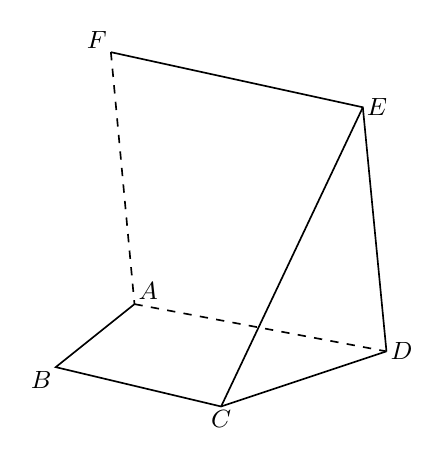
\begin{tikzpicture}[semithick, every node/.style={inner sep=1.2pt, font=\small}]
  \coordinate (F) at (0.2,4.4);
  \coordinate (E) at (3.4,3.7);
  \coordinate (A) at (0.5,1.2);
  \coordinate (D) at (3.7,0.6);
  \coordinate (B) at (-0.5,0.4);
  \coordinate (C) at (1.6,-0.1);
  \draw (F) -- (E) -- (D);
  \draw[dashed] (F) -- (A);
  \draw (A) -- (B) -- (C) -- (D);
  \draw[dashed] (A) -- (D);
  \draw (C) -- (E);
  \node[above left] at (F) {$F$};
  \node[right] at (E) {$E$};
  \node[above right] at (A) {$A$};
  \node[right] at (D) {$D$};
  \node[below left] at (B) {$B$};
  \node[below] at (C) {$C$};
\end{tikzpicture}
